\chapter{Theoretical Background}
\label{chap2}
\section{Fundamentals of Bearing Fault Frequencies}
{
\subsection{Overview}
{
The most significant challenge that the authors had to deal with is that of the faulty cases detection. For this reason, fault and unfault models have been developed, and series of comparisons between the actual model generated by apparatus measurements and these two situational models are being executed. This development constitutes a real challenge since this is the main criterion that identifies the state of the motor.
}

\subsection{Unfault and Fault Models}
{
As previously mentioned, the authors make use of a model-based approach, which entails that the main concept is comparison-oriented. Specifically, there is the unfault model, which contains a high-amplitude peak at the shaft rotating frequency $F_{\omega}$. In addition to that, it can be noticed in Figure~\ref{fig:faultsunfaults} that some other patterns distinct themselves from the previously-mentioned unfault model. Regarding the unbalance model, it is obvious that the amplitude at the first tone is much greater. In the case of the misalignment model, it can be noticed that the tone at $2F_{\omega}$ has a much greater amplitude while the amplitude at the tone of the shaft speed $F_{\omega}$ remains at a high level. In the case of looseness, there are some more tones prevailing on the spectrum, among the tones related to the shaft speed. To top it all off, the most important vibration spectrum is that of the bearing failure (Refer to Figure~\ref{fig:faultTree}). Every bearing is characterized by four critical frequencies, given by its manufacturer, and these frequencies are associated with the four bearing components (inner and outer ring, balls, and cage):

\begin{itemize}
	\item BPFO (Ball Pass Frequency Outer) - outer race failure
	\item BPFI (Ball Pass Frequency Inner) - inner race failure
	\item BSF (Ball Spin Frequency) - rolling element failure
	\item FTF (Fundamental Train Frequency) - cage failure
\end{itemize}

\begin{figure}[h]
\centering
\includegraphics[width=\linewidth]{figures/FaultsAndUnfaults.png}
\caption{Fault and unfault spectrum graphs \cite{Betta2002}.}
\label{fig:faultsunfaults}
\end{figure}

\begin{figure}[h]
	\centering
	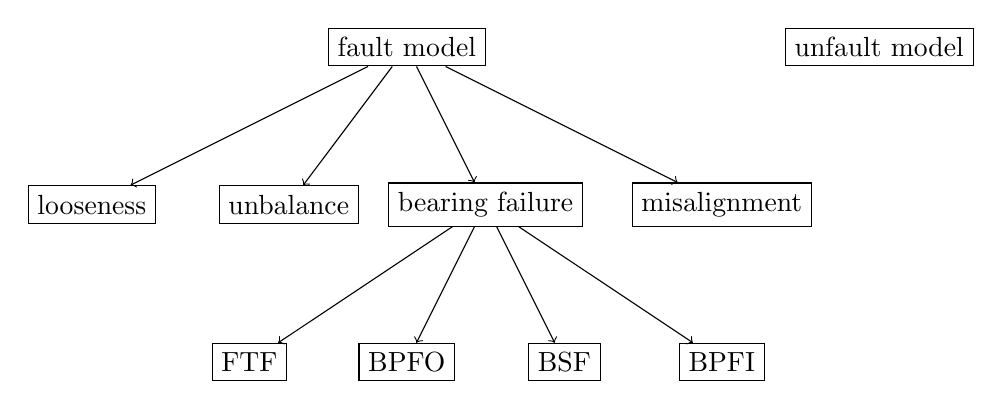
\begin{tikzpicture}
		\node (box1) [draw, rectangle] at (0,0) {unfault model};
		\node (box2) [draw, rectangle, left of=box1, node distance=6cm] {fault model};
 		\node (box3) [draw, rectangle] at (-7.5,-2) {unbalance};
		\node (box4) [draw, rectangle] at (-2,-2) {misalignment};
		\node (box5) [draw, rectangle] at (-5,-2) {bearing failure};
		\node (box6) [draw, rectangle] at (-10,-2) {looseness};
		\node (box7) [draw, rectangle] at (-6,-4) {BPFO};
		\node (box8) [draw, rectangle] at (-2,-4) {BPFI};
		\node (box9) [draw, rectangle] at (-4,-4) {BSF};
		\node (box10) [draw, rectangle] at (-8,-4) {FTF};
		
		% Arrows
		\draw[->] (box2) -- (box3);
		\draw[->] (box2) -- (box4);
		\draw[->] (box2) -- (box5);
		\draw[->] (box2) -- (box6);
		\draw[->] (box5) -- (box7);
		\draw[->] (box5) -- (box8);
		\draw[->] (box5) -- (box9);
		\draw[->] (box5) -- (box10);
	\end{tikzpicture}
	\caption{Unfault and fault model sub-categories} \label{fig:faultTree}
\end{figure}

It is also worth noting that a fault-emulation method can be used in such cases to simulate the faulty models. This entails that additional tones can be stressed, and crucial spectra modifications may take place for research and comparison purposes.
}


}




\section{Algorithms and Technologies}
% Summary of FFT, data flow, etc.
\subsection{Signal Processing}
\subsubsection{Fast Fourier Transform (FFT)}
{

The Cooley-Tukey algorithm (1965) is a divide-and-conquer method that provides a fast algorithm for computing the complex Fourier transform efficiently:
\[
X_j = \sum_{k=0}^{n-1} x_k \exp\left( \frac{i2\pi jk}{n} \right) \quad \text{for} \quad j = 0,1,\dots,n-1,
\]

This reduces complexity from $\mathcal{O}(n^2)$ (naive DFT) to $\mathcal{O}(n \log n)$, enabling major time savings for complex and large-scale transforms. The algorithm is implemented in major numerical packages including MATLAB and NumPy's FFT routines.
}

\subsection{Embedded Systems \& IoT}
\subsubsection{ADXL335 Sensor}
Analog signal from sensor breakout to arduino. To elaborate on signal transferring
\begin{itemize}
\item what a sensor breakout is
\item what analog signal is
\end{itemize}


\subsubsection{Arduino Microcontroller}
UART serial communication sending data to RPi. To elaborate on this protocol
\begin{itemize}
\item what serial protocol is
\item what Arduino is
\end{itemize}

\subsubsection{Raspberry Pi 4}
RPi receiving data using a script and posing HTTP Post data to a supabase api. Elaborate on this

\begin{itemize}
\item how to collect data and analyse
\item what Raspberry Pi 4 is
\end{itemize}




\subsection{Backend \& Database}
\subsubsection{Supabase}
\begin{itemize}  
	\item PostgreSQL. 
	\item APIs
	\item what http post is
\end{itemize}  

\subsubsection{Vercel and Next.js}
\begin{itemize}  
	\item nextjs 
	\item vercel
\end{itemize} 